\pdfvariable minorversion=7
\pdfvariable inclusioncopyfonts=1

\documentclass{arialFHGR} % use either arialFHGR or timesFHGR
\newcommand{\haupttitel}{Masterthesis}
\newcommand{\untertitel}{Implementierung einer webbasierten 3D-Terrainvisualisierung auf Basis von swisstopo-Daten und eines Quadtree basierten LOD-Systems}
\newcommand{\zusammenfassung}{Abstract}
\newcommand{\autorenschaft}{Yannick Hutter}
\newcommand{\studiengang}{Msc User Experience Design \& Data Visualization}
\newcommand{\matrikelnummer}{17-175-829}
\newcommand{\adresse}{Talackerstrasse 8}
\newcommand{\ort}{Mels}
\newcommand{\plz}{8887}
\newcommand{\department}{Departement]}
\newcommand{\institute}{Schweizerisches Institut für Informationswissenschaft (SII)}
\newcommand{\modul}{Masterthesis HS25}
\newcommand{\email}{yannick.hutter@stud.fhgr.ch}
\newcommand{\refe}{Prof. Dr. habil. Wolfgang Semar}
\newcommand{\coRefe}{Franjo Pehar}
\newcommand{\abgabedatum}{27.02.2026}
\newcommand{\abgabedatumRFC}{2025-11-29}
\newcommand{\sprache}{de}
\newcommand{\schlagworte}{}

\input{config/preamble}
\begin{document}

    \renewcommand{\contentsname}{Inhaltsverzeichnis}
    \renewcommand{\listfigurename}{Abbildungsverzeichnis}
    \renewcommand{\listtablename}{Tabellenverzeichnis}
    \renewcommand{\acronymname}{Abkürzungsverzeichnis}
    \renewcommand{\lstlistlistingname}{\texorpdfstring{Programmcodeverzeichnis\bigskip}{Programmcodeverzeichnis}}
    
    
    \pagenumbering{Roman}

    \input{content/01_vorspann/01.1_titelblatt}
    \include{content/01_vorspann/01.2_abstract}

    \tableofcontents 
        
    % List of figures
    \cleardoublepage
    \phantomsection
    \addcontentsline{toc}{chapter}{\listfigurename}
    \listoffigures
    
    % List of tables
    \cleardoublepage
    \phantomsection
    \addcontentsline{toc}{chapter}{\listtablename}
    \listoftables

    % List of acronyms
    \printglossary[type=\acronymtype]
    \cleardoublepage
    \newpage
    
    \pagenumbering{arabic}
    \chapter{Einleitung}
\label{chap_einleitung}
In der heutigen Zeit gibt es viele verschiedene Möglichkeiten, Datenvisualisierungen auf interaktive Art und Weise zugänglich zu machen. Nebst der Darstellungsdimensionalität (2D/3D) spielt auch die eingesetzte Technologie eine entscheidende Rolle. Mit dem Aufkommen von immersiven Technologien wie \acrfull{VR} und \acrfull{CAVE} gibt es viele Optionen, die Daten für den Nutzer explorierbar zu machen. Der Fokus der vorliegenden Masterarbeit ist die Darstellung von Daten im dreidimensionalen Raum, wobei ein immersives Erlebnis im Vordergrund steht. Konkret hat sich die Arbeit zum Ziel gesetzt, eine 3D Terrain Visualisierung auf Basis von swisstopo-Daten für das \acrshort{CAVE}-System der \acrfull{FHGR} zu implementieren. Die Visualisierung soll hierbei in Echtzeit exploriert werden können. Im Rahmen der Arbeit sollen folgende Forschungsfragen geklärt werden:
\begin{itemize}
    \item Welche Technologie ist für eine echtzeitfähige 3D Datenvisualisierung geeignet?
    \item Welche Algorithmen sind für eine echtzeitfähige 3D Datenvisualisierung von Gebirgen geeignet?
    \item Welche Probleme treten bei der Datenvorverarbeitung auf?
    \item Welche Probleme treten bei der 3D Datenvisualisierung von Gebirgen auf?
    \item Wie kann die Ästhetik einer 3D Datenvisualisierung beeinflusst werden?
    \item Welche Optimierungen sind notwendig, um die Echtzeitfähigkeit der Visualisierung zu gewährleisten?
\end{itemize}

Der thematische Aufbau der Arbeit orientiert sich an den oben stehenden Forschungsfragen und gliedert sich wie folgt auf. Kapitel \ref{chap_datengrundlage} befasst sich mit den zugrundeliegenden Daten der Visualisierung. Kapitel \ref{chap_technologien} zeigt auf welche bestehenden Technologien es gibt, um Daten auf effiziente Weise in 3D darzustellen. Kapitel \ref{chap_render_pipelines} erläutert wichtige Terminologien und schafft ein notwendiges Grundverständnis, wie 3D-Rendering im Allgemeinen funktioniert. Kapitel \ref{chap_algorithmen} veranschaulicht wichtige Algorithmen, um die Echtzeitfähigkeit zu gewährleisten. In Kapitel \ref{chap_swiss_terrain_3d}  geht es um die eigentliche Implementierung der Terrainvisualisierung. Hierbei wird auf wichtige Aspekte wie die Datenvorverarbeitung, die genutzten Algorithmen, auftretende Problematiken sowie Optimierungen eingegangen. Anschliessend erfolgt in Kapitel \ref{chap_diskussion} eine Diskussion der Arbeit mit Bezug auf die oben definierten Forschungsfragen. Abgerundet wird die Arbeit durch Kapitel \ref{chap_ausblick}, welches einen Ausblick über mögliche Erweiterungen der Visualisierung und nicht thematisierte Aspekte behandelt.

    \chapter{Datengrundlage}
\label{chap_datengrundlage}
TODO
    \chapter{Technologien zur Erstellung von 3D Computergrafiken}
\label{chap_technologien}
Dieses Kapitel bietet einen Überblick über die Technologielandschaft zur Erstellung von 3D Computergrafiken. Konkret wird auf populäre Spiele Engines wie Unity, Godot sowie Unreal Engine eingegangen. Nebst den Engines werden auch verschiedene Frameworks wie ThreeJS, CelsiumJs sowie sokol thematisiert. Zu guter Letzt wird noch auf immersive Technologien wie \acrshort{VR} sowie \acrshort{CAVE} eingegangen.

\section{Engines}
Engines sind umfassende Programme, welche das Erstellen von 3D Computergrafiken und insbesondere Videospielen für jedermann zugänglich machen. Anders als Frameworks beinhalten diese Programme bereits integrierte Editoren, welche das Erstellen von 3D-Welten und interaktiven Erlebnissen vereinfachen. Für viele komplexe Systeme wie Physik und Audio werden des Weiteren fertige Komponenten zur Verfügung gestellt. Wie bei normalen Programmen gibt es auch bei Spiele Engines kostenlose und kostenpflichtige Varianten. Nachfolgend wird auf die populärsten 3D-fokussierten Engines in beiden Bereichen eingegangen.  

\subsection{Unity Engine}
Rückblickend auf das Jahr 2024 bezogen ist die Unity Engine die meistgenutzte Spiele Engine für kleinere bis mittelgrosse 3D Erlebnisse (siehe Abbildung \ref{fig_nutzung_spiele_engines}). Unity gehört zu den kostenpflichtigen Spiele Engines und unterstützt rund 20 verschiedene Plattformen. Angefangen bei den klassischen Desktop-Betriebssystemen wie MacOS, Linux und Windows über Webbrowser bis zu verschiedenen Spielekonsolen und VR-Headsets \parencite{unity_platform_support_2025}.
\begin{figure}[H]
    \caption{Übersicht Nutzung Spiele Engine nach Spielgrösse \parencite[S. 7]{vgi_report_2025}}
    \includegraphics[width=.5\linewidth]{content/00_assets/uebersicht_nutzung_spielengines.png}
    \label{fig_nutzung_spiele_engines}
\end{figure}

Die Spiele selbst werden in Unity innerhalb des Unity-Editors (siehe Abbildung \ref{fig_unity_editor}) und mithilfe der Programmiersprache C-Sharp entwickelt. 
\begin{figure}[H]
    \caption{Unity Editor \parencite{unity_editor_2019}}
    \includegraphics[width=.5\linewidth]{content/00_assets/unity_editor.jpg}
    \label{fig_unity_editor}
\end{figure}

Je nach Funktionsumfang gibt es verschiedene Lizenzmodelle bei Unity. Das Lizenzmodell ist hierbei nicht nur vom Funktionsumfang, sondern auch vom Jahreseinkommen abhängig (siehe Tabelle \ref{table_unity_preise}). Für das Erstellen von industriellen Anwendungen muss zudem eine spezielle ``Industry-Lizenz'' erworben werden (Preis auf Anfrage).
\begin{table}[H]
    \caption{Lizenzkosten der Unity Engine in Abhängigkeit zum Jahreseinkommen \parencite{unity_preise_2025}}
    \begin{tabularx}{\textwidth} {
        >{\raggedright\arraybackslash}X 
        >{\raggedright\arraybackslash}X
        >{\raggedright\arraybackslash}X}
            \hline
            \textbf{Lizenzmodell} & {Jahreseinkommen} & {Jahreskosten}  \\
            \hline
            Personal & weniger als 200'000 USD & {Gratis}\\
            Pro & zwischen 200'000 USD und 25'000'000 USD & 2'220 USD pro Nutzer \\
            Enterprise & mehr als 25'000'000 USD &  auf Anfrage \\
            \hline
    \end{tabularx}
    \bigbreak
    \label{table_unity_preise}
\end{table}

\subsection{Unreal Engine}
Über die Jahre haben viele Spielentwicklungsstudios bekannt gegeben, dass sie ihre eigens entwickelte Engine durch die Unreal Engine ersetzen werden \parencite[S. 11]{vgi_report_2025}. Unreal Engine zeichnet sich durch die beeindruckenden visuellen Effekte aus. Sie wird jedoch nicht nur zur Entwicklung von Videospielen eingesetzt, sondern kommt auch im Rahmen von Filmproduktionen sowie Architekturvisualisierungen (siehe Abbildung \ref{fig_unreal_engine_architektur}) zum Einsatz. Insbesondere im Architekturbereich werden hierbei gängige Datenformate wie \acrfull{BIM} \parencite{unreal_engine_architektur_2025} unterstützt.
\begin{figure}[H]
    \caption{Unreal Engine Achitektur Visualisierung \parencite{unreal_engine_architektur_2025}}
    \includegraphics[width=.5\linewidth]{content/00_assets/unreal_engine_achitektur.png}
    \label{fig_unreal_engine_architektur}
\end{figure}

Unreal Engine gehört ebenfalls zu den kommerziellen Spiele Engines. Beim Lizenzmodell wird zwischen zwei verschiedenen Kategorien unterschieden. Werden Videospiele erstellt, so ist eine kostenlose Nutzung bis zu einem Umsatz von einer Million USD möglich. Danach müssen jeweils 5\% des Gewinns als Lizenzkosten abgegeben werden. Werden hingegen Produkte abseits von Videospielen entwickelt, so fallen nach der ersten Million rund 1'800 USD an jährlichen Lizenzgebühren an \parencite{unreal_engine_lizenzkosten_2025}. 

Nebst einem integrierten Editor werden von Unreal Engine zahlreiche Tools für die Erstellung von immersiven Erlebnissen angeboten. Mithilfe des World Partitioning Tools können beispielsweise riesige 3D-Welten erstellt werden. Hierbei wird die virtuelle Welt anhand eines Gitternetzes in dedizierte Teilbereiche unterteilt. Während sich der Nutzer durch die Welt bewegt, werden diese Bereiche anschliessend dynamisch gestreamt \parencite{unreal_engine_2025}. Auch beim Erstellen von 3D Modelle wird Hand geboten. Quixel Megascan erlaubt das Integrieren von 3D Modellen mithilfe von fotogrammetrischen Verfahren sowie die Nutzung von hochauflösenden Texturen \parencite{unreal_engine_quixel_2025}. Die eigentliche Logik der 3D Visualisierungen wird in Unreal mithilfe der systemnahen Programmiersprache C++ sowie einer visuellen Scriptsprache namens ``Blueprints'' umgesetzt. Blueprints erlaubt es, komplexe Funktionalitäten mithilfe von Nodes und entsprechenden Verbindungen umzusetzen (siehe Abbildung \ref{fig_unreal_engine_blueprints}). Dies erlaubt es auch Personen ohne entsprechende Programmierkenntnisse, verschiedene Ideen auszuprobieren, wohingegen komplexe Aspekte in C++ implementiert werden können. 
\begin{figure}[H]
    \caption{Unreal Engine Blueprints \parencite{unreal_engine_blueprints_2026}}
    \includegraphics[width=.5\linewidth]{content/00_assets/unreal_engine_blueprints.png}
    \label{fig_unreal_engine_blueprints}
\end{figure}

\subsection{Godot Engine}
Nebst kommerziellen Spiele Engines wie Unity und Unreal gibt es auch komplett kostenlose Alternativen wie die Godot Engine. Die Engine basiert auf der MIT Open Source Lizenz und bietet uneingeschränkte Nutzungsrechte sowie Zugriff auf den gesamten Quellcode \parencite{godot_mit_license_2023}.  
Godot benötigt im Vergleich zu Unity und Unreal Engine auch signifikant weniger Speicherplatz. Für die Engine werden lediglich zwischen 200MB und 1.5GB Festplattenspeicher benötigt. Dies ist eine erhebliche Reduktion im Vergleich zu den 5 - 20GB der Unity sowie den 30 bis 50GB der Unreal Engine. Wie Unity und Unreal unterstützt auch Godot diverse verschiedene Plattformen. Von den bekannten Betriebssystemen wie MacOS, Linux und Windows über Webbrowser bis zu mobilen Endgeräten wird ein breites Spektrum abgedeckt \parencite{godot_faq_2025}. Ebenso verfügt Godot über einen integrierten Editor, welcher die Erstellung von 3D-Welten erleichtert. Aufgrund der freizügigen MIT Lizenz gibt es darüber hinaus diverse weitere Tools, welche auf der Engine selbst basieren. Mithilfe von Material Maker können beispielsweise prozedurale Texturen erstellt werden (siehe Abbildung \ref{fig_godot_material_maker}). Mithilfe der App Xogot kann Godot sogar auf Apple Geräten wie dem iPhone oder iPad verwendet werden \parencite{godot_xogot_2025}.
\begin{figure}[H]
    \caption{Material Maker Tool zur Erzeugung von prozeduralen Texturen \parencite{godot_material_maker_2025}}
    \includegraphics[width=.5\linewidth]{content/00_assets/godot_material_maker.png}
    \label{fig_godot_material_maker}
\end{figure}

\section{Frameworks}
Anders als Engines besitzen Frameworks in der Regel keinen integrierten Editor. Stattdessen werden einzelne Bausteine und Programmiermodule für wichtige Funktionalitäten wie 3D Rendering, Audio und Physik Systeme angeboten. Aufgrund des reduzierten Umfangs in Hinblick auf Funktionalität, Tooling sowie unterstützte Plattformen sind Frameworks auch leichtgewichtiger und ressourcenschonender als komplette Spiele Engines. Jedoch ist auch der Programmierer selbst dafür verantwortlich, die einzelnen Bausteine zu einer Gesamtlösung zu kombinieren. Hierdurch entsteht grosser Handlungsfreiraum in Hinblick auf Softwarearchitektur und Funktionsweise. Jedoch müssen auch entsprechende technische Grundlagen vorhanden sein.

\subsection{Three.js}
Mit über 3 Millionen Downloads pro Woche zählt Three.js zu den populärsten webbasierten Frameworks für 3D-Grafiken \parencite{threejs_downloads_2025}. Das Framework basiert wie die Godot Engine auf der MIT Open Source Lizenz und kann daher ohne Bedenken und Einschränkungen für Projekte aller Art verwendet werden \parencite{threejs_lizenz_2024}. Anders als Unity, Unreal und Godot ist die primäre Zielplattform von Three.js der Browser. Browserbasierte Anwendungen haben den Vorteil, dass keinerlei Installation der Software notwendig ist und gleichzeitig ein breites Spektrum von Endgeräten abgedeckt werden kann. Hierbei werden vom Framework moderne Browser-Grafikschnittstellen wie WebGL2 sowie WebGPU unterstützt. Diese Grafikschnittstellen erlauben die Umsetzung von detailreichen und performanten 3D-Anwendungen. Three.js abstrahiert und vereinheitlicht auch Unterschiede in der Implementierung der Grafikschnittstellen zwischen den einzelnen Browsern. Hierdurch werden Browserinkompatibilitäten von 3D-Anwendungen vermieden. Nebst einer umfangreichen Dokumentation\footnote{\url{https://threejs.org/manual/}} stehen über 150 verschiedene Beispielprojekte\footnote{\url{https://threejs.org/examples/}} zur Verfügung. Auch internationale Unternehmen wie Apple setzten bereits Three.js auf der eigenen Webseite ein, um Produkte wie das iPhone in 3D zu bewerben. Das Framework kann aber auch dazu eingesetzt werden, um komplette interaktive und erlebbare 3D-Welten zu erschaffen, wie das Portfolio von Simon Bruno zeigt (siehe Abbildung \ref{fig_threejs_portfolio_simon_bruno}).
\begin{figure}[H]
    \caption{Interaktives Portfolio von Simon Bruno \parencite{threejs_simon_bruno_portfolio_2025}}
    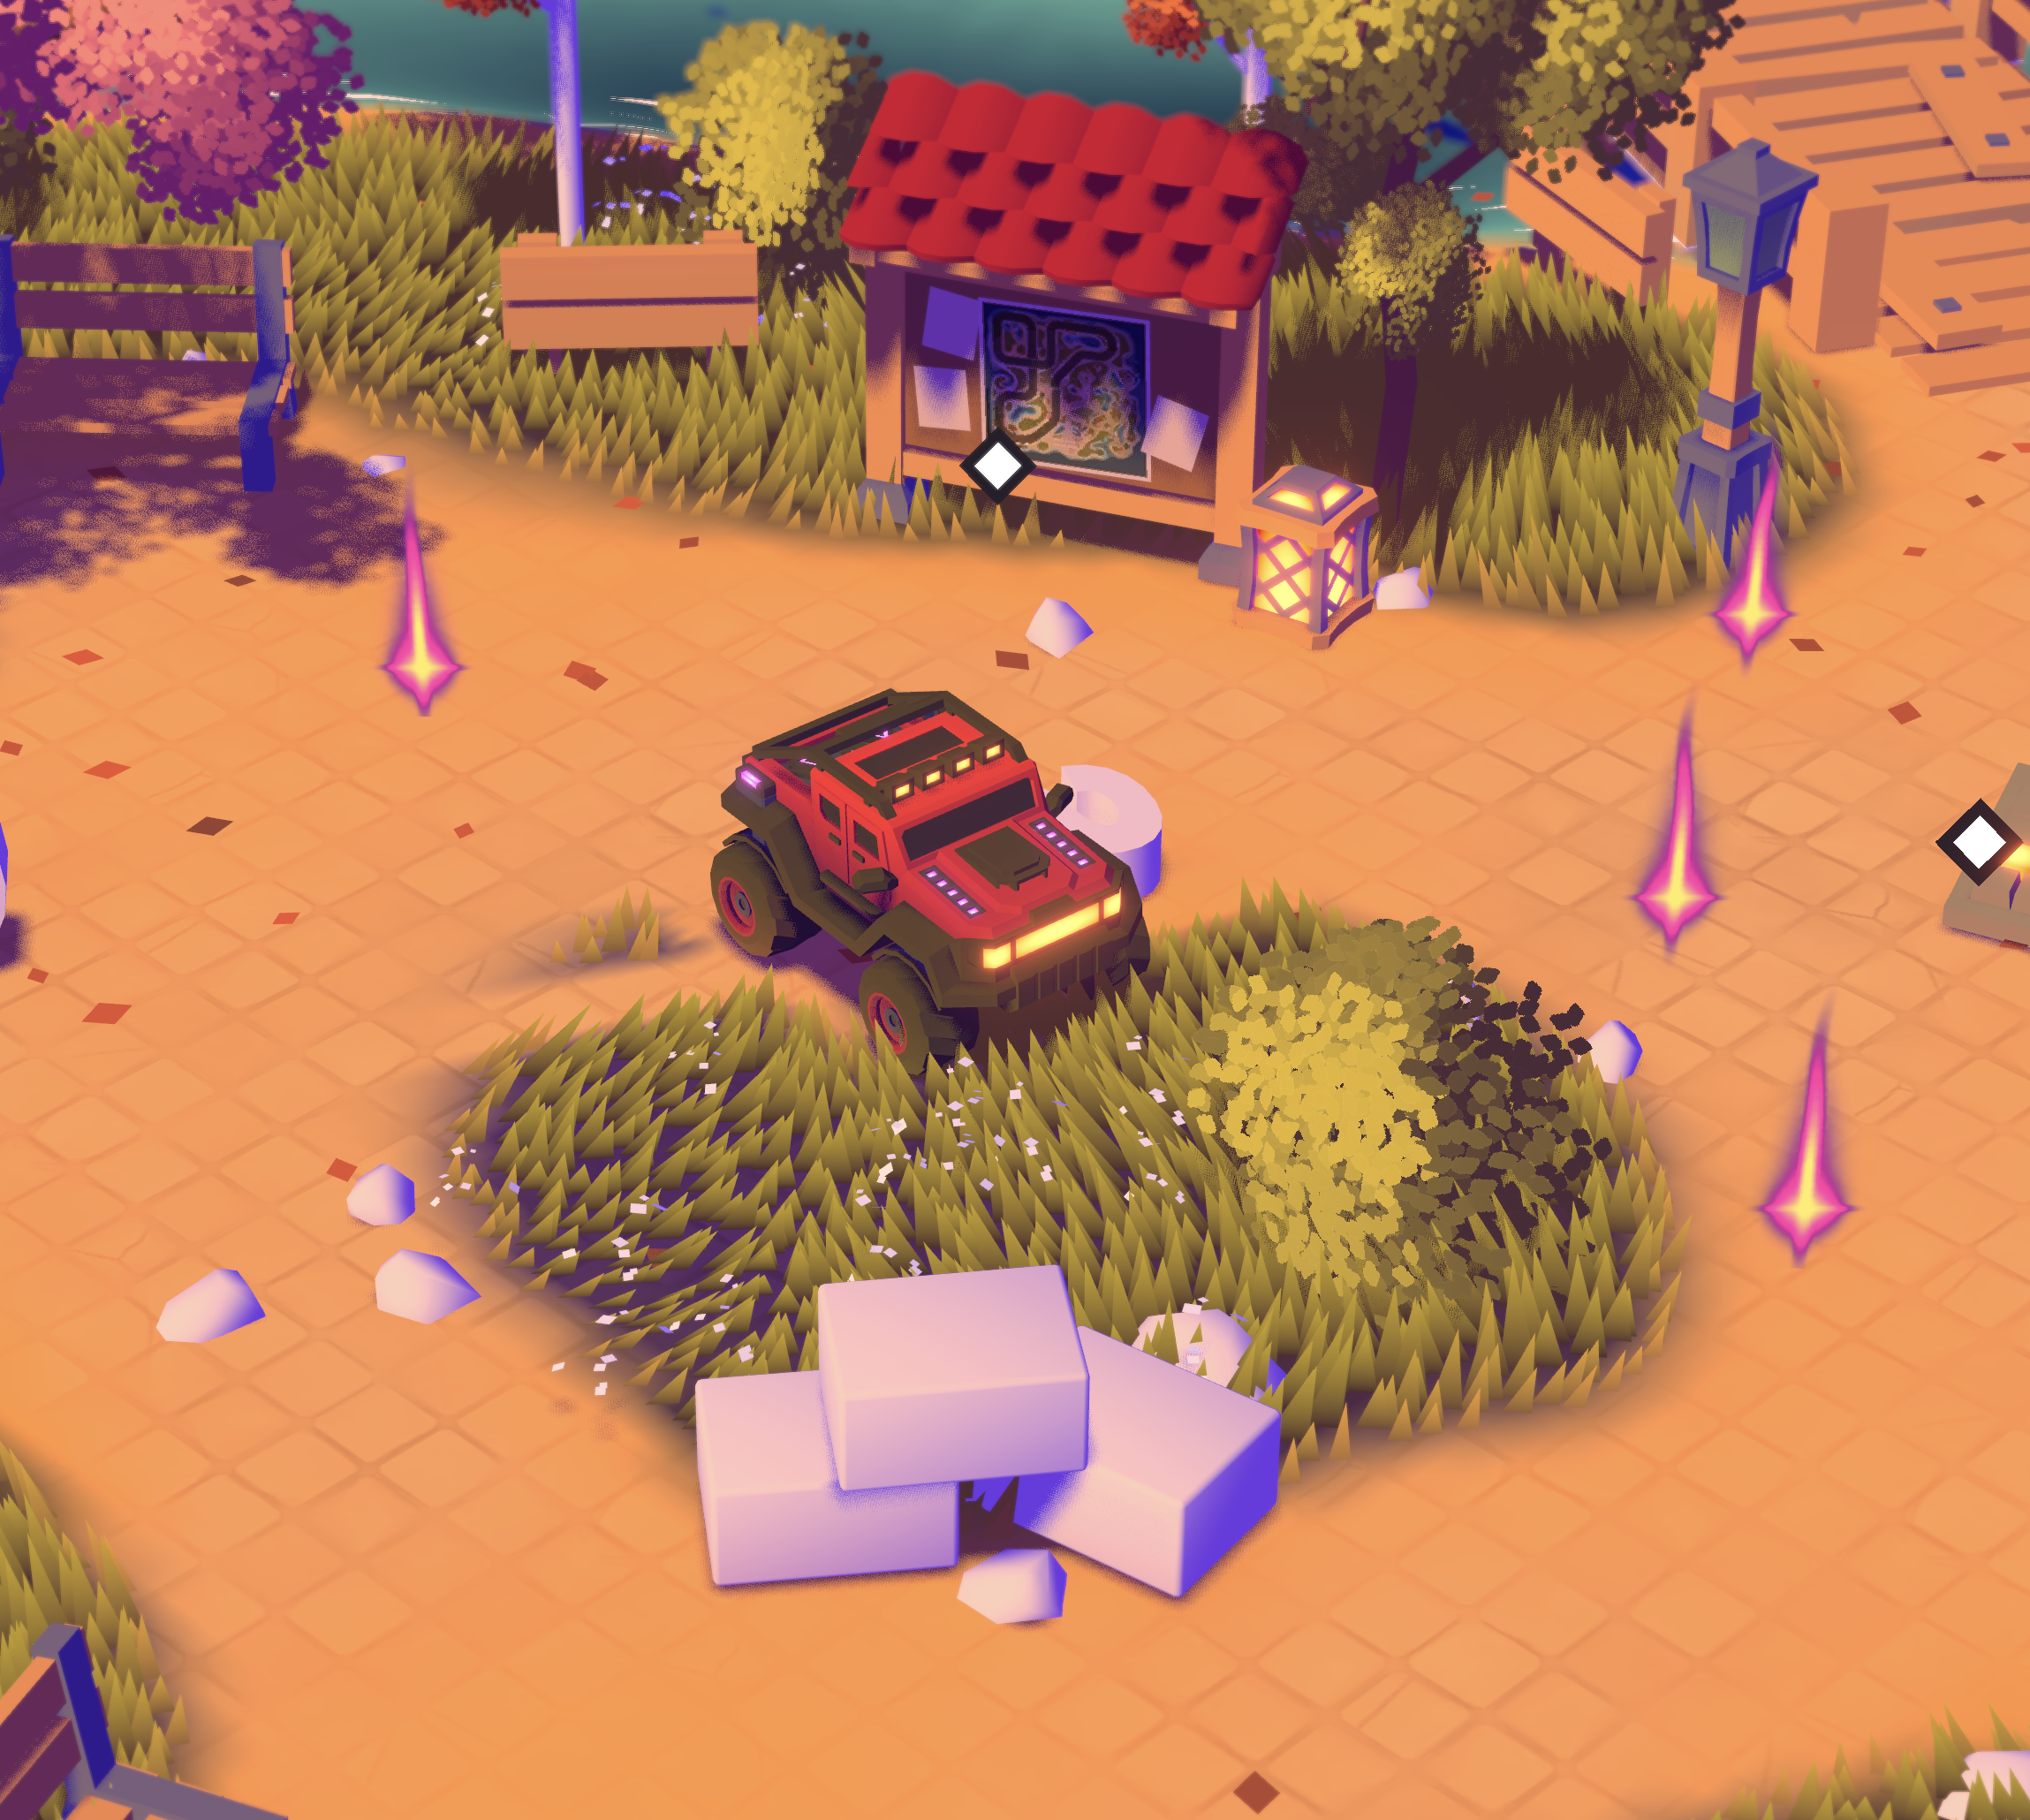
\includegraphics[width=.4\linewidth]{content/00_assets/threejs_portfolio_simon_bruno.png}
    \label{fig_threejs_portfolio_simon_bruno}
\end{figure}

Three.js kann auch dazu eingesetzt werden, um komplette browserbasierte VR-Anwendungen mittels WebXR umzusetzen. Die primäre Programmiersprache des Frameworks ist JavaScript. Jedoch können auch Sprachen mit statischer Typisierung wie TypeScript\footnote{\url{https://www.typescriptlang.org/}} ohne Probleme verwendet werden. 

\subsection{Babylon.js}
Nebst Three.js ist auch Babylon.js ein sehr prominentes Webframework. Babylon.js wurde im Jahr 2013 von Microsoft basierend auf der Programmiersprache TypeScript entwickelt. Wie Three.js werden sowohl die WebGL2 als auch WebGPU Grafikschnittstelle unterstützt. Im Gegensatz zu Three.js besitzt Babylon.js eine integrierte Physik-Engine, einen Inspektor (siehe Abbildung \ref{fig_babylonjs_inspektor}) sowie einen UI-Editor \parencite{babylonjs_gui_editor_2025}. All diese Features machen Babylon.js zu einem populären Webframework, welches rund 14'600 mal pro Woche heruntergeladen wird \parencite{babylonjs_npm_2025}. Die Downloadgrösse beträgt hierbei rund 60MB und ist somit rund doppelt so gross wie jene von Three.js. Wie Three.js hat auch Babylon.js eine umfassende Dokumentation\footnote{\url{https://doc.babylonjs.com/}}. Im Gegensatz zu Three.js, welches einen modularen und weitestgehend freizügigen Strukturaufbau erlaubt, gibt Babylon.js in vielen Bereichen die Struktur und Art und Weise vor, wie gewisse Probleme zu lösen sind \parencite{babylonjs_vs_threejs_2025}. Aufgrund der Apache 2.0 Open Source Lizenz kann das Framework ohne Bedenken für kommerzielle Zwecke eingesetzt werden \parencite{babylonjs_lizenz_2025}.
\begin{figure}[H]
    \caption{BabylonJs Inspektor \parencite{babylonjs_inspector_2025}}
    \includegraphics[width=.4\linewidth]{content/00_assets/babylonjs_inspektor.png}
    \label{fig_babylonjs_inspektor}
\end{figure}

\subsection{Sokol}
Anders als browserbasierte Anwendungen, laufen native Applikationen direkt auf dem entsprechenden Betriebssystem  und können auch ohne Internetverbindung genutzt werden. Jedes Betriebssystem verwendet hierbei jedoch eine andere Grafikschnittstelle. Unter Windows wird primär DirectX verwendet, wohingegen unter Linux OpenGL sowie Vulkan und bei MacOS die Metal Grafikschnittstelle zum Einsatz kommen. Soll eine Applikation auf allen Betriebssystemen unterstützt werden, muss diese daher für jede Grafikschnittstelle einzeln entwickelt werden. Sokol\footnote{\url{https://github.com/floooh/sokol}} ist ein Framework, welches verschiedene Grafikschnittstellen abstrahiert und vereinheitlicht. Dies hat den Vorteil, dass die Anwendung nur einmal entwickelt werden muss. Sokol basiert auf der Open Source ZLib Lizenz und kann daher kostenfrei für kommerzielle Projekte eingesetzt werden. Das Framework ist in der systemnahen Programmiersprache C geschrieben und daher besonders performant und speichereffizient. Es stehen diverse Tools zur Verfügung, welche das Arbeiten mit den 3D-Grafikschnittstellen vereinfachen. Mithilfe des ``Shader Code Generator Tool'' \footnote{\url{https://github.com/floooh/sokol-tools/blob/master/docs/sokol-shdc.md}} (sokol-shdc) können Shader für unterschiedliche Grafikschnittstellen generiert werden (eine detailliertere Erklärung zu Shader folgt in Kapitel \ref{chap_render_pipelines}). Nebst den bekannten Betriebssystemen wird auch der Browser als mögliche Zielplattform unterstützt. Hierzu wird \acrfull{Wasm} verwendet, um C-Code in eine assemblerähnliche Sprache für den Browser zu übersetzen. \acrshort{Wasm} hat den Vorteil, dass der generierte Code eine geringe Dateigrösse aufweist und in einer effizienten Art und Weise ausgeführt werden kann. Wie Three.js besitzt Sokol einen modularen Aufbau. Die einzelnen Module stehen als sogenannte ``Single Header Library'' zur Verfügung. Das bedeutet, dass sich der gesamte Code eines Moduls in einer einzelnen Datei befindet und keine Abhängigkeiten auf andere Dateien besitzt. Dies erleichtert die Integration in ein bestehendes Projekt, da jeweils nur eine Datei integriert werden muss und kein komplexes Build-System notwendig ist. Die Dokumentation selbst befindet sich in Form von Quellcode-Kommentaren ebenfalls in den entsprechenden Single Header Libraries. Wie in Three.js bietet auch Sokol diverse Beispiele an, welche auch direkt im Browser angeschaut werden können (siehe Abbildung \ref{fig_sokol_beispiele}).
\begin{figure}[H]
    \caption{Sokol Beispiele \parencite{sokol_beispiele_2025}}
    \includegraphics[width=.6\linewidth]{content/00_assets/sokol_beispiele.png}
    \label{fig_sokol_beispiele}
\end{figure}

\subsection{Electron}
\label{chap_electron}
Es wurden sowohl webbasierte als auch native Frameworks thematisiert. Webbasierte Frameworks haben im Gegensatz zu den nativen Frameworks den Vorteil, dass keine Installation notwendig ist und sie auf einem breiten Spektrum von Endgeräten lauffähig sind. Ein Nachteil von Webframeworks ist jedoch ein sehr eingeschränkter Zugriff auf Dinge wie Multithreading sowie auf das Dateisystem.

Electron\footnote{\url{https://www.electronjs.org/}} ist ein Framework, mithilfe dessen browserbasierte Anwendungen direkt auf dem entsprechenden Betriebssystem als native Anwendungen ausgeführt werden können. Hierzu kombiniert Electron die eigentliche Webanwendung mit einem Chromium Browser und einer entsprechenden Node.js Runtime zu einer nativen Anwendung \parencite{electron_documentation_2025}. Hierdurch erhöht sich zwar der Festplattenverbrauch im Vergleich zu einer komplett nativen Anwendung, jedoch erlangen Browseranwendungen so auch Zugriff auf wichtige native Funktionalitäten wie Kamera und Dateisystem \parencite{electron_why_2025}. Die Verwendung von Electron aufgrund der Open Source MIT Lizenz komplett kostenfrei und uneingeschränkt möglich \parencite{electron_license_2021}.

\subsection{Tauri}
Tauri\footnote{\url{https://v2.tauri.app/}} besitzt wie Electron das Ziel, browserbasierte Anwendungen als native Applikationen auf dem Betriebssystem auszuführen. Anders als Electron verpackt Tauri jedoch nicht einen kompletten Browser in die native Anwendung, sondern benutzt sogenannte ``WebViews''. WebViews sind Softwarekomponenten, welche das Einbinden von browserbasierten Inhalten in nativen Anwendungen erlauben und auf allen gängigen Betriebssystemen vorhanden sind. Anders als vollwertige Browser benötigen WebViews auch um ein Vielfaches weniger Festplattenspeicher. Eine auf Tauri basierte Anwendung kann somit auf bis zu 600KB reduziert werden. Vergleicht man diesen Wert mit den sonst benötigten 80 - 150MB bei einer Electron Anwendung ergibt sich hierdurch eine signifikante Ersparnis des Festplattenverbrauches. Unternehmen wie Microsoft verwenden WebViews bereits in den eigenen Produkten wie Microsoft Teams \parencite{microsoft_teams_webview_2023}. Um den Zugriff auf native Betriebssystemfunktionalitäten zu ermöglichen, benutzt Tauri verschiedene Module, welche in der systemnahen Programmiersprache Rust geschrieben sind. Ein Nachteil von WebViews im Gegensatz zu kompletten Browsern wie Chromium besteht darin, dass Unterschiede in den angebotenen Funktionalitäten je nach Betriebssystem auftreten können. Wenn jedoch Festplattenspeicher wie auch eine ressourcenschonendere Anwendung im Vordergrund stehen, ist Tauri eine ansprechende Alternative zu Electron.

\section{Immersive Technologien}
Frameworks und Engines helfen dabei, ansprechende 3D-Erlebnisse zu gestalten. Um jedoch ein immersives Erlebnis zu gewährleisten, reicht das alleine oft nicht aus. Technologien wie \acrshort{VR} und \acrshort{CAVE}-Systeme helfen dabei, die Immersion für den Nutzer komplett zu machen und ihm das Gefühl zu vermitteln, dass er sich mitten des virtuellen Erlebnisses befindet.

\subsection{\acrfull{VR}}
Bei klassischen 3D Anwendungen befindet sich der Nutzer in der Regel vor einem Bildschirm. \acrshort{VR} funktioniert anders. Anstelle eines Bildschirms werden ein \acrshort{VR}-Headset sowie entsprechende Controller verwendet (siehe Abbildung \ref{fig_vr_headset_controller}). Dies sorgt für ein besonders immersives Erlebnis. Mithilfe der Controller kann der Nutzer sich durch die virtuelle Welt bewegen und mithilfe des Headsets die Blickrichtung komplett frei bestimmen. Um ein immersives Erlebnis zu gewährleisten, muss hierfür jedoch auch entsprechend viel Bewegungsfreiraum vorhanden sein. Zudem müssen die Geräte entsprechend kalibriert werden. Moderne Browser und Webframeworks wie Three.js und Babylon.js erlauben es, VR-Anwendungen direkt innerhalb des Browsers mithilfe der WebXR\footnote{\url{https://immersiveweb.dev/}}-API umzusetzen. VR-Anwendungen sind hierdurch nicht nur auf native Plattformen und mobile Endgeräte beschränkt und erhalten eine noch breitere Reichweite und Adaption.
\begin{figure}[H]
    \caption{Person mit VR-Headset und Controller \parencite{vr_headset_controller}}
    \includegraphics[width=.3\linewidth]{content/00_assets/vr_headset_controller.jpg}
    \label{fig_vr_headset_controller}
\end{figure}

\subsection{\acrfull{CAVE}}
\label{chap_cave}
Anders als bei \acrshort{VR} ist bei einem \acrshort{CAVE}-System kein Headset notwendig. Für ein CAVE-System benötigt es einen Raum, in dem sich der Nutzer frei bewegen kann, entsprechende Projektoren und Rechner. Der Nutzer befindet sich in der Mitte des Raums, während auf die Wände die Visualisierung projiziert wird \parencite{cave_1992}. Dies gibt der Person das Gefühl, dass sie sich inmitten der Visualisierung befindet. Ein Vorteil von CAVE besteht darin, dass einfach mit Personen kollaboriert werden kann. Mehrere Personen können sich gleichzeitig im selben Raum befinden und miteinander über wichtige Aspekte der Visualisierung diskutieren (siehe Abbildung \ref{fig_cave_collaboration}). Vorallem im Bildungsbereich und in wissenschaftlichen Visualisierungen ein grosser Vorteil \parencite{cave_collaboration_2020}.
\begin{figure}[H]
    \caption{Kollaboration in einem CAVE-System \parencite[S. 11]{cave_collaboration_2020}}
    \includegraphics[width=.5\linewidth]{content/00_assets/cave_collaboration.png}
    \label{fig_cave_collaboration}
\end{figure}

 Jedoch sind die Anschaffungskosten eines professionellen CAVE-Systems im Vergleich zu VR-Systemen höher. Nebst dem eigentlichen Raum werden mehrere Projektoren, Rechner und weitere Hardware benötigt. Ebenso wird entsprechende Software benötigt, welche die Visualisierung verzerrungsfrei und synchron auf alle Wände projiziert. Ein bewährtes Konzept, um dies zu bewerkstelligen, ist das sogenannte ``Master-Slave'' Prinzip \parencite{Flynn2014CAVE}. Pro Wand gibt es einen entsprechenden Rechner und Projektor. Auf jedem Rechner läuft die gleiche Visualisierung. Einer der Rechner (Master) gibt den Takt zur Synchronisierung vor und übermittelt die notwendigen Synchronisationsdaten (Kameraposition etc.) an die anderen Rechner (Slave). Die Slaves visualisieren jeweils ihren eigenen Ausschnitt der Visualisierung in Abhängigkeit von den Synchronisationsdaten und dem vorgegebenen Takt.
 
 Ein CAVE-System kann mit entsprechender Hardware beliebig erweitert werden. Mithilfe von Head Tracking Hardware ist das dynamische Verfolgen der Person im Raum möglich. Hiermit kann sich die Visualisierung dynamisch anhand der Position anpassen und so neue Blickwinkel eröffnen. Aufgrund des breiten Spektrums an Erweiterungsmöglichkeiten ergeben sich auch unterschiedliche Preissegmente, angefangen bei vierstelligen bis zu hohen siebenstelligen Beträgen. Für die Inbetriebnahme der CAVE-Systeme gibt es entsprechend spezialisierte Firmen wie Inside Reality\footnote{\url{https://inside-reality.com/product/icroom/}}, welche nebst der entsprechenden Software auch die entsprechende Hardware und Expertise anbieten.
    \chapter{Render Pipelines}
\label{chap_render_pipelines}
TODO
    \chapter{Algorithmen}
\label{chap_algorithmen}
TODO
    \chapter{Datenvorverarbeitung}
\label{chap_datenvorverarbeitung}
TODO
    \chapter{Swiss Terrain 3D}
\label{chap_swiss_terrain_3d}
TODO
    \chapter{Optimierungen}
\label{chap_optimierungen}
TODO
    \chapter{Ausblick}
\label{chap_ausblick}
Im Rahmen dieses Kapitels werden der aktuelle Stand, bestehende Limitationen sowie entsprechende Lösungsansätze der Terrainvisualisierung thematisiert. Ebenso werden weiterführende Optimierungs- sowie Erweiterungsmöglichkeiten für die Zukunft aufgezeigt.


\section{Aktueller Stand}
Während dieser Arbeit wurde eine webbasierte, echtzeitfähige Terrainvisualisierung  auf Basis der swisstopo Datensätze umgesetzt. Die Basis hierzu bildet eine weitestgehend komplett automatisierte Datenvorverarbeitung. Der Nutzer muss lediglich die gewünschte Region auf der offiziellen swisstopo-Webseite auswählen und die entsprechende CSV-Datei herunterladen. Anschliessend werden im Rahmen der Datenvorverarbeitung automatisch die entsprechenden Datensätze heruntergeladen, Lücken geschlossen sowie entsprechende Texturen in unterschiedlichen Auflösungen und Metadaten generiert. Die vorverarbeiteten Daten werden zur Laufzeit anhand der Metadaten sowie einer Quadtree Datenstruktur in entsprechende 3D Geometrien umgewandelt. Diese 3D Geometrien werden anschliessend zu einem Gebirge zusammengesetzt. Der Nutzer hat die Möglichkeit, sich mithilfe von verschiedenen Steuerungselementen durch das Gebirge zu bewegen. Während sich der Nutzer fortbewegt, werden der Quadtree sowie das Terrain abhängig von der Position aktualisiert und entsprechend verfeinert. Entsprechende UI-Elemente erlauben es dem Nutzer, das Aussehen sowie die Ästhetik des Terrains in Echtzeit anzupassen.

\section{Limitationen und Lösungsansätze}
Obwohl mithilfe der Quadtree Datenstruktur sowie entsprechend vorgenommenen Optimierungen eine echtzeitfähige Terrainvisualisierung auf Basis der swisstopo Datensätze umgesetzt werden konnte, bestehen noch gewisse Limitationen. Eine Hauptlimitation ist die Beschränkung auf einen quadratischen Ausschnitt des Gebirges. Diese Entscheidung wurde vom Autor getroffen, um sicherzustellen, dass die in der Datenvorverarbeitung erzeugten Texturen ebenfalls eine quadratische Auflösung besitzen. Der Grund für diese Entscheidung ist der Umstand, dass Grafikkarten prinzipiell Texturen in einer quadratischen Auflösung bevorzugen. Jedoch können sowohl die Quadtree Datenstruktur als auch die Grafikkarte ebenso mit nicht quadratischen Texturen umgehen. Hierdurch könnte das gesamte Gebirge visualisiert werden und wäre nicht auf einen Teilausschnitt limitiert.

Eine weitere Limitierung besteht in der Auflösung der Datensätze. Momentan werden sowohl für den swissALTI3D als auch swissIMAGE Datensatz die gleiche Auflösung von 2 Meter pro Bildpunkt verwendet. Ein Kilometer hat somit eine Auflösung von 500px auf 500px. Jedoch stehen beide Datensätze in weiteren Auflösungen zur Verfügung. Da die Datensätze auf dem LV95-Koordinatensystem basieren, sollte es daher möglich sein, unterschiedliche Auflösungen für die Höhen sowie Bilddaten zu verwenden und höher aufgelöste Gebirgsstrukturen zu erhalten. Dies ist insbesondere für Bildschirme mit hoher Auflösung oder CAVE-Systeme mit entsprechend grossen Projektionsflächen von Relevanz. Jedoch müsste hierbei je nach Einsatzzweck die Grösse der Datenmengen beachtet werden. Auf einer Webseite, wo schnelle Ladezeiten eine wichtige Rolle spielen, sollten kleinere Auflösungen und somit kleinere Datensätze präferiert werden. Im Rahmen eines CAVE-Systems ist jedoch eine längere Startphase für höhere und detailgetreuere Darstellungen eher verkraftbar.

Eine letzte Limitierung, welche auffällt, wenn sich der Nutzer durch das Gebirge fortbewegt, ist das plötzliche Erscheinen neuer Geometrien. Dieser Effekt, auch bekannt unter dem Begriff ``Pop-in-Effekt'' kann störend wirken, primär dann, wenn neue Geometrien in der unmittelbaren Nähe des Betrachters erzeugt werden und aus dem Nichts erscheinen. Ein Lösungsansatz hierzu ist das sogenannte ``Vertex Morphing'', welches auch Filip Strugar in seinem Paper verwendet \parencite[S. 7]{strugar_cdlod_2009}. Die Idee hinter dem Vertex Morphing ist es, die einzelnen Punkte zwischen verschiedenen Geometrien anhand eines Morph Faktors zu interpolieren. Hiermit kann ein fliessender Übergang zwischen den 3D Geometrien erreicht werden. Für die Terrainvisualisierung könnte beispielsweise zwischen Geometrien unter LOD-Stufen interpoliert werden. Als Morph Faktor für die Interpolation kann die gleiche Metrik wie beim Quadtree verwendet werden, sprich der Abstand von der Kamera zum Mittelpunkt der einzelnen Geometrien. 

\section{Optimierungspotenzial}
Kapitel \ref{chap_future_optimizations} zeigte Optimierungsmöglichkeiten in Bezug auf das 3D Rendering mithilfe von Techniken wie Instance Rendering auf. Darüber hinaus gibt es jedoch noch weiteres Optimierungspotenzial.  

Eine Optimierungsmöglichkeit besteht in der Nutzung von Frustum Culling für den Quadtree Algorithmus selbst. Momentan wird das komplette Gebirge mithilfe des Quadtree Algorithmus unterteilt. Jedoch könnte bereits während der Generierung des Quadtrees das Sichtfeld der Kamera berücksichtigt und somit die Laufzeitkomplexität des Algorithmus weiter reduziert werden.

Wie in Kapitel \ref{chap_compute_shader} angesprochen sind Compute Shader eine Möglichkeit, um generelle Berechnungen auf der Grafikkarte auszuführen. Hierdurch könnte beispielsweise sowohl das Frustum Culling, welches von Three.js auf der CPU ausgeführt wird, als auch der Quadtree Algorithmus komplett auf die Grafikkarte ausgelagert werden. Anders als die CPU wird die Arbeit auf der GPU hierbei parallel ausgeführt. Bei grossen Gebirgen sollten die notwendigen Berechnungen daher um Faktoren schneller erledigt werden können. Um die Auswirkungen von Compute Shader auf die Laufzeitkomplexität zu erfassen, müssten jedoch auch entsprechende Tests mit unterschiedlichsten Gebirgsgrössen durchgeführt werden.

\section{Zukünftige Erweiterungsmöglichkeiten}
Die Terrainvisualisierung wurde als webbasierte Lösung entwickelt und ist daher ohne Installationsaufwand auf einer Vielzahl von unterschiedlichen Plattformen lauffähig. Eine mögliche Zielplattform ist ein \textbf{CAVE-System} (siehe Kapitel \ref{chap_cave}).

CAVE-Systeme haben grössere Projektionsflächen als herkömmliche Computermonitore. Deshalb ist es wichtig, entsprechend hochaufgelöste Texturen zu verwenden. Hierzu müsste das Python-Script für die Datenvorverarbeitung entsprechend angepasst werden, sodass Datensätze mit einer unterschiedlichen Auflösung verarbeitet werden können. Nebst grösseren Auflösungen besitzen CAVE-Systeme in der Regel auch mehrere Computer. Jeder Computer projiziert hierbei die Visualisierung auf eine separate Projektionsfläche. Deshalb ist es wichtig, die Visualisierung zwischen den verschiedenen Computern synchron zu halten. Hierzu könnten die notwendigen Informationen wie Kameraposition, Blickwinkel und Rotation mithilfe von Websockets zwischen den Rechnern in Echtzeit ausgetauscht werden.

Da die Visualisierung mithilfe des Frameworks Three.js implementiert wurde, stehen auch Technologien wie Web-VR zur Verfügung. Hiermit wäre auch eine Umsetzung als \textbf{Virtual Reality Anwendung} im Browser möglich. Selbstverständlich müssten dann jedoch auch technische Aspekte wie Steuerungselemente, welche momentan mittels Maus und Tastatur funktionieren, überarbeitet werden.

Generell könnten die Steuerungselemente erweitert werden, sodass eine Vielzahl von unterschiedlichen Eingabegeräten unterstützt wird. Mithilfe von 3D-Mäusen wäre etwa die Fortbewegung im dreidimensionalen Raum komplett ohne Tastatur und herkömmlicher Maus umsetzbar. Durch Bibliotheken wie mediapipe\footnote{\url{https://github.com/google-ai-edge/mediapipe}} ist auch die Erkennung von Handgestenbewegungen in Echtzeit möglich. Hierdurch würden sich auch weitere Eingabemöglichkeiten ergeben.

Die Ausweitung auf Systeme wie CAVE oder VR in Kombination mit verschiedenen Interaktionsmöglichkeiten und Steuerungselementen würde sich auch für einen Nutzertest im Bereich Usability Engineering eignen. Hierbei könnten nebst den eigentlichen Interaktionselementen auch die Ästhetik und deren Auswirkungen untersucht werden.

Momentan ist zwar die Datenvorverarbeitung mithilfe eines Python-Skripts automatisiert, jedoch muss dieses vom Nutzer entsprechend ausgeführt werden. Eine Erweiterung in diesem Bereich ist das Integrieren der Datenvorverarbeitung in die Anwendung selbst. Dem Nutzer könnte hierzu in der Anwendung selbst eine Liste mit Regionen angezeigt werden. Nach der Auswahl einer Region wird automatisch die entsprechende CSV-Datei heruntergeladen und die Datenvorverarbeitung gestartet. Mithilfe von Frameworks wie Electron und Tauri (siehe Kapitel \ref{chap_electron}) könnte zudem die webbasierte Anwendung als eigenständige Applikation direkt auf dem Rechner des Nutzers umgesetzt werden. Dies hätte den Vorteil, dass die Anwendung auch offline ausgeführt werden könnte.

Nebst den Datensätzen swissALTI3D und swissIMAGE bietet swisstopo auch einen swissSURFACE3D Datensatz\footnote{\url{https://www.swisstopo.admin.ch/de/hoehenmodell-swisssurface3d-raster}} an. Dieser Datensatz beinhaltet wie swissALTI3D ebenfalls ein digitales Oberflächenmodell jedoch werden hierbei auch Boden, Bewuchs, Wälder, Hochbauten und weitere Kunstbauten einbezogen \parencite{swissSURFACE3D_2024}. Mithilfe dieser Informationen könnten die Gebirge mit weiteren Objekten wie Wäldern und Bebauungen erweitert werden. Mithilfe von Shadern könnten hierzu noch entsprechende Wolkengebilde und Seen generiert werden, was wiederum die Ästhetik der Anwendung verbessert.

    
    \printbibliography[heading=bibintoc,title={Literaturverzeichnis}]
    \chapter*{Hilfsmittelverzeichnis}
\addcontentsline{toc}{chapter}{Hilfsmittelverzeichnis}
\begin{table}[H]
    \begin{tabularx}{\textwidth} {
        >{\raggedright\arraybackslash}X 
        >{\raggedright\arraybackslash}X 
        >{\raggedright\arraybackslash}X}
            \hline
            \textbf{Hilfsmittel} & \textbf{Verwendungszweck} & \textbf{Quelle}  \\
            \hline
            Three.js Journey & Online-Kurs für das Three.js Framework & \url{https://threejs-journey.com} \\
            Simon Dev GLSL Course & Online-Kurs für GLSL-Shader & \url{https://simondev.teachable.com/p/glsl-shaders-from-scratch} \\
            Carbon & Erstellung Screenshots für Code-Snippets & \url{https://carbon.now.sh} \\
            Github & Git-Repository & \url{https://github.com/yhutter/swiss-terrain-3d} \\
            LaTeX Vorlage FHGR & Dokumentenvorlage & \url{https://github.com/giodi/Vorlage-FHGR} \\
            \hline
    \end{tabularx}
    \bigbreak
\end{table}
    \appendix
    \chapter{Anhang}

\section{Element 1}

    \chapter*{Eiderklärung}
\addcontentsline{toc}{chapter}{Eiderklärung}

Ich erkläre hiermit, dass ich diese Arbeit selbstständig verfasst und keine anderen als die angegebenen Quellen und erlaubten Hilfsmittel benutzt habe, einschliesslich der Verwendung von KI-Systemen. Alle Stellen, die wörtlich oder sinngemäss aus Quellen entnommen worden sind, habe ich als solche gekennzeichnet. Ich bin den Vorgaben des Leitfadens wissenschaftliches Arbeiten gefolgt. Mir ist bekannt, dass andernfalls die Hochschulleitung zum Entzug der aufgrund meiner Arbeit verliehenen Qualifikation oder des für meine Arbeit verliehenen Titels berechtigt ist.

\noindent \includegraphics[height=2cm]{content/00_assets/unterschrift.png}
    
\end{document}